\documentclass[UTF8,zihao=-4]{ctexart}

\usepackage[a4paper,left=2.35cm,right=2.35cm,top=2.35cm,bottom=2.35cm]{geometry}
\usepackage{amsmath,amssymb}
\usepackage{booktabs,longtable,array,multirow}
\usepackage{enumitem}
\usepackage{xcolor}
\usepackage{hyperref}
\usepackage{url}
\usepackage{listings}
\usepackage{caption}
\usepackage{graphicx}
\usepackage{fancyhdr}

\hypersetup{
  colorlinks=true,
  linkcolor=blue!60!black,
  citecolor=blue!60!black,
  urlcolor=blue!60!black
}

\pagestyle{fancy}
\fancyhf{}
\lhead{协程技术调研}
\rhead{\thepage}
\setlength{\headheight}{14.5pt}

\setlist[itemize]{leftmargin=2em,itemsep=0.25em,topsep=0.25em}
\setlist[enumerate]{leftmargin=2em,itemsep=0.25em,topsep=0.25em}

\lstset{
  basicstyle=\ttfamily\small,
  breaklines=true,
  frame=single,
  columns=fullflexible,
  keepspaces=true,
  showstringspaces=false,
  keywordstyle=\color{blue!70!black},
  commentstyle=\color{green!40!black},
  stringstyle=\color{orange!70!black}
}

\title{\heiti 协程技术调研报告：从并发模型演进到底层实现}
\author{姓名：匡航逸 \quad 学号：2412235}
\date{\today}

\begin{document}
\maketitle

\begin{abstract}
随着云端服务并发度不断提高，传统“一个请求对应一个操作系统线程”的模型在高并发 I/O 场景下会受到线程栈、内核调度、上下文切换和线程池排队等成本限制。协程技术的核心思想是：把“等待”从“占用线程”中分离出来，让一个任务在遇到 I/O、定时器或同步点时主动或透明地挂起，并在条件满足后由运行时恢复执行。本文围绕协程产生的背景、协程的语义模型、编译器与运行时实现、操作系统配合机制，以及 C++20、Go、Python、C\#、Java 21 等主流语言中的协程或轻量级线程支持展开调研。最后给出本机可复现实验：一组构造大量可挂起等待任务，另一组使用纯 Python 循环构造 CPU 密集负载，用于说明协程与线程池的性能边界。
\end{abstract}

\noindent\textbf{关键词：} 协程；异步编程；事件循环；非阻塞 I/O；Goroutine；async/await；虚拟线程；运行时调度

\tableofcontents
\newpage

\section{问题背景：为什么并发模型会演进到协程}

\subsection{并发需求的变化}

在传统单机程序中，任务数量通常较少，程序主要关心如何充分利用 CPU。进入互联网和云服务时代后，大量服务变成了典型的 I/O 密集型系统，例如 Web 服务器、RPC 网关、数据库代理、爬虫、消息队列消费者等。这类程序的特点是：

\begin{itemize}
  \item 请求数量很多，但每个请求大部分时间不是在计算，而是在等待网络、磁盘、数据库或下游服务；
  \item 单个任务的 CPU 使用率不高，但并发任务数量可能达到几千、几万甚至更多；
  \item 如果每个请求都绑定一个操作系统线程，线程栈和内核调度开销会迅速变成瓶颈。
\end{itemize}

因此，协程的出现不是偶然的。它试图解决的不是“单个任务如何算得更快”，而是“系统如何在大量任务都在等待时，仍然保持较低资源占用和较高吞吐”。

\subsection{从进程、线程到协程的演进}

可以把并发执行机制的演进概括为以下路线：

\begin{center}
\begin{tabular}{p{3cm}p{5.2cm}p{5.8cm}}
\toprule
阶段 & 优点 & 主要问题 \\
\midrule
多进程 & 隔离性好，一个进程崩溃不一定影响其他进程 & 创建和切换开销大，进程间通信成本高 \\
多线程 & 共享地址空间，通信方便，能利用多核 & 每个线程通常对应内核调度实体，线程栈和上下文切换成本较高 \\
线程池 & 限制线程数量，避免无限制创建线程 & 大量阻塞任务会占满线程池，导致排队和吞吐下降 \\
事件驱动 / 回调 & 单线程可管理大量 I/O，资源开销低 & 控制流被拆散，回调嵌套严重，错误处理和调试困难 \\
协程 / async-await & 保留接近同步代码的写法，同时具备异步 I/O 的伸缩性 & 需要语言、运行时和库共同配合；阻塞调用、取消传播、调试仍需注意 \\
虚拟线程 / Goroutine & 接近线程式编程体验，但单位任务更轻量 & 运行时复杂度提高；CPU 密集任务仍受核心数限制 \\
\bottomrule
\end{tabular}
\end{center}

Linux 上现代 pthread 实现 NPTL 相比早期 LinuxThreads 具有更好的 POSIX 符合性和大规模线程创建性能，但它仍然是以操作系统线程为基础的模型\cite{pthreads}。协程进一步向前走了一步：把大量用户态任务映射到较少的内核线程上，使运行时可以更细粒度地控制任务挂起、恢复和调度。

\section{协程的基本概念}

\subsection{协程是什么}

通俗地说，协程是“可以暂停和恢复的函数”。普通函数一旦被调用，就沿着调用栈执行到返回；协程则可以在中间的某个挂起点保存自己的执行状态，把控制权交回调用者或调度器，之后再从挂起点继续运行。

C++20 文档中对协程的描述非常直接：协程是能够挂起执行并在之后恢复的函数。C++20 协程是 stackless coroutine，也就是不保存完整线程栈，而是把恢复所需的数据保存在单独的 coroutine state 中\cite{cppref}。

协程的关键组成包括：

\begin{itemize}
  \item \textbf{挂起点}：例如 \texttt{await}、\texttt{co\_await}、\texttt{yield} 等；
  \item \textbf{协程帧}：保存局部变量、参数、当前执行位置等；
  \item \textbf{恢复句柄或 continuation}：调度器通过它恢复协程；
  \item \textbf{调度器 / 事件循环}：决定哪个协程现在可以继续执行；
  \item \textbf{I/O 事件源}：如 epoll、kqueue、IOCP、定时器、Future 完成事件等。
\end{itemize}

\subsection{协程、线程、异步 I/O 的区别}

\begin{center}
\begin{tabular}{p{3.2cm}p{4.2cm}p{6.5cm}}
\toprule
概念 & 调度者 & 特点 \\
\midrule
操作系统线程 & 操作系统内核 & 可被内核抢占，能利用多核，但栈和调度成本较高 \\
用户态协程 & 语言运行时或库 & 创建和切换轻量，通常在挂起点协作式让出执行权 \\
异步 I/O & 操作系统 + 运行时 & I/O 发起后不阻塞当前线程，完成后通过事件通知恢复任务 \\
线程池 & 运行时或框架 & 复用有限数量线程，但阻塞任务仍会占用线程 \\
事件循环 & 运行时库 & 维护 ready queue、timer queue 和 I/O poller，适合 I/O 密集型 \\
\bottomrule
\end{tabular}
\end{center}

一个重要理解是：\textbf{协程不是异步 I/O 本身，而是让异步 I/O 更容易写的一种控制流表达方式。} 早期事件驱动模型也可以实现高并发，但它通常需要手写回调；协程和 \texttt{async/await} 的价值在于，编译器或运行时把“回调链”重新包装成“看起来像顺序执行的代码”。

\section{协程的应用范式}

协程并不是把所有并发问题都简化成“创建很多任务”。在工程实践中，协程通常和限流、队列、超时、取消传播等机制一起使用。较常见的范式包括：

\begin{itemize}
  \item \textbf{请求级协程}：Web 服务、RPC 网关或代理程序中，一个请求对应一个协程。请求处理逻辑可以保持接近顺序代码，但数据库查询、下游 RPC、缓存读取等等待点会挂起当前协程，把执行线程让给其他请求。
  \item \textbf{fan-out / fan-in}：一个上层请求需要同时访问多个下游服务时，可以把多个子请求拆成协程并发发出，再用 \texttt{gather}、\texttt{join} 或类似机制汇总结果。这类模式能降低总等待时间，但必须设置超时和失败策略。
  \item \textbf{生产者--消费者流水线}：爬虫、日志处理、消息消费等场景中，不同阶段通过异步队列连接。生产者负责产生 URL、消息或数据块，消费者并发处理；队列长度和消费者数量构成天然的背压控制。
  \item \textbf{受限并发}：协程很轻量，但下游数据库、文件描述符、连接池和第三方服务并不无限。实际程序通常需要信号量、连接池、令牌桶或 bounded queue，避免“协程很多”变成“请求风暴”。
  \item \textbf{超时、取消和结构化并发}：高并发程序中，父任务取消时应能传播到子任务；部分子任务失败时应明确决定继续、重试还是整体失败。否则协程虽然轻量，也会留下难以追踪的后台任务。
\end{itemize}

这些范式的共同点是：协程负责表达大量可挂起的控制流，运行时负责调度，工程代码仍然要显式管理容量、生命周期和错误边界。

\section{协程的底层实现机制}

\subsection{核心思想：把函数调用改写成状态机}

以 \texttt{async/await} 为例，编译器通常会把一个异步函数拆成状态机。每遇到一个 \texttt{await}，函数就可能被分割为多个状态：

\begin{itemize}
  \item \textbf{状态 0}：从函数入口执行到第一个 \texttt{await}；
  \item \textbf{状态 1}：第一个等待对象完成后，从第一个 \texttt{await} 后继续；
  \item \textbf{状态 2}：第二个等待对象完成后继续；
  \item \textbf{结束状态}：返回结果或抛出异常。
\end{itemize}

挂起时，运行时需要保存：
\begin{itemize}
  \item 当前执行到哪个状态；
  \item 跨越挂起点仍然存活的局部变量；
  \item 返回值、异常、取消状态；
  \item 后续恢复时要执行的 continuation。
\end{itemize}

这解释了为什么协程可以“暂停”。它并不神秘，本质是把执行现场从线程栈上搬到一个可保存、可恢复的数据结构中。

\subsection{C++20 中的协程帧、promise 和 awaiter}

C++20 协程由 \texttt{co\_await}、\texttt{co\_yield}、\texttt{co\_return} 触发。C++ 标准库只提供底层机制，不直接规定完整的事件循环或网络异步库。

一个 C++20 协程通常涉及三个重要概念\cite{cppref}：

\begin{itemize}
  \item \textbf{promise object}：协程内部通过它提交返回值或异常；
  \item \textbf{coroutine handle}：协程外部通过它恢复或销毁协程帧；
  \item \textbf{coroutine state}：保存 promise、参数、挂起点信息以及跨挂起点存活的局部变量。
\end{itemize}

\texttt{co\_await expr} 大致会调用三个方法：

\begin{enumerate}
  \item \texttt{await\_ready()}：判断结果是否已经就绪；如果已就绪，可以不挂起；
  \item \texttt{await\_suspend(handle)}：真正挂起当前协程，并把恢复句柄交给调度器、线程池或 I/O 回调；
  \item \texttt{await\_resume()}：协程恢复后取得结果或抛出异常。
\end{enumerate}

因此，C++20 给的是“可挂起函数”的底层抽象。至于协程什么时候恢复、在哪个线程恢复、如何与 epoll 或 IOCP 对接，需要由库或框架实现。

\subsection{事件循环：协程运行时的心脏}

以 Python \texttt{asyncio}、Node.js/libuv 或很多 C++ 异步框架为例，事件循环通常维护三类结构：

\begin{itemize}
  \item \textbf{ready queue}：已经可以立即运行的任务；
  \item \textbf{timer heap}：到时间后需要唤醒的任务；
  \item \textbf{I/O poller}：等待文件描述符、socket 或系统完成事件。
\end{itemize}

一个简化的事件循环可以写成：

\begin{lstlisting}[language=Python,caption={简化事件循环伪代码}]
while not stopped:
    run_all_ready_tasks()

    timeout = time_until_next_timer()
    events = io_poller.wait(timeout)

    for event in events:
        task = event_to_task[event]
        ready_queue.push(task)

    move_expired_timers_to_ready_queue()
\end{lstlisting}

Python 官方文档指出，\texttt{asyncio} 的事件循环是每个 asyncio 应用的核心，用于运行异步任务、回调、执行网络 I/O 和子进程操作\cite{asyncio-eventloop}。在 \texttt{asyncio.Task} 的说明中，官方文档也明确提到：事件循环采用协作式调度，一个事件循环一次运行一个 Task；当一个 Task 等待 Future 完成时，事件循环可以运行其他 Task、回调或执行 I/O 操作\cite{asyncio-task}。

\subsection{操作系统如何配合：非阻塞 I/O 和事件通知}

协程本身运行在用户态，但真正的网络 I/O、文件描述符状态变化仍然需要操作系统支持。Linux 上常见机制是 \texttt{epoll}，BSD/macOS 上常见机制是 \texttt{kqueue}，Windows 上常见机制是 IOCP。libuv 文档说明，其事件循环采用单线程异步 I/O 方式：网络 I/O 使用非阻塞 socket，并在不同平台上使用最佳的轮询机制，例如 Linux 上的 epoll、macOS/BSD 上的 kqueue、Windows 上的 IOCP\cite{libuv}。

以 Linux epoll 为例，协程运行时一般做以下事情：

\begin{enumerate}
  \item 将 socket 设置为非阻塞；
  \item 协程调用异步读操作；
  \item 如果当前没有数据，系统调用返回 \texttt{EAGAIN}；
  \item 运行时把当前协程挂起，并把 fd 注册到 epoll；
  \item epoll 等到 fd 可读后返回事件；
  \item 运行时把对应协程放回 ready queue；
  \item 协程恢复，继续执行读操作之后的逻辑。
\end{enumerate}

Linux \texttt{epoll(7)} 手册也强调，边缘触发模式下通常应结合非阻塞文件描述符使用，并在 \texttt{read} 或 \texttt{write} 返回 \texttt{EAGAIN} 后再等待事件\cite{epoll}。

\section{主流语言中的协程支持对比}

\subsection{整体对比表}

{\small
\setlength{\tabcolsep}{3pt}
\begin{longtable}{@{}p{2.1cm}p{2.55cm}p{3.0cm}p{3.55cm}p{3.15cm}@{}}
\toprule
语言 / 平台 & 编程接口 & 调度模型 & 优势 & 注意点 \\
\midrule
C++20 & \texttt{co\_await}, \texttt{co\_yield}, \texttt{co\_return} & 标准只提供 stackless coroutine 机制；调度器由库实现 & 零成本抽象潜力大，可深度定制 awaiter、promise、executor & 标准库层面缺少统一事件循环和网络异步抽象，工程复杂度较高 \\
\midrule
Go & \texttt{go f()}，channel & Goroutine 映射到 OS thread；runtime 使用 G-M-P 模型 & 语法简单，运行时自动调度，适合服务端高并发 & 阻塞、GC、调度公平性、共享内存竞争仍需理解 \\
\midrule
Python & \texttt{async def}, \texttt{await}, \texttt{asyncio} & 单事件循环内协作式调度 Task & 适合网络 I/O，生态成熟，代码可读性好 & CPU 密集型受 GIL 和单事件循环限制；阻塞函数会卡住事件循环 \\
\midrule
C\#/.NET & \texttt{async}/\texttt{await}, \texttt{Task} & 编译器生成状态机；Continuation 通常由 TaskScheduler/线程池调度 & 与 .NET 任务模型结合紧密，异常处理和组合 API 完整 & \texttt{async void}、上下文捕获、同步阻塞 \texttt{Result/Wait} 容易造成问题 \\
\midrule
Java 21 & Virtual Threads & JVM 用户态线程，挂载到 carrier platform thread 上执行 & 保留同步阻塞风格，大幅降低 thread-per-request 成本 & 不是 CPU 加速工具；synchronized/native 等 pinning 场景可能影响伸缩性 \\
\bottomrule
\end{longtable}
}

\subsection{C++20：底层机制强，但需要库补全}

C++20 协程适合需要极致控制的场景。它的特点是：
\begin{itemize}
  \item 协程是 stackless 的，保存的是协程帧而不是完整调用栈；
  \item \texttt{co\_await} 的语义由 awaiter 控制；
  \item 协程恢复点、局部变量、promise 等保存在 coroutine state 中；
  \item 可以与线程池、事件循环、网络库、生成器等机制结合。
\end{itemize}

C++20 的优势是抽象开销可控，适合系统软件和高性能网络框架；缺点是标准层面提供的是底层砖块，不是开箱即用的 async runtime。也就是说，C++20 协程更像是“编译器级 continuation 支持”，而不是完整的应用层并发框架。

\subsection{Go：Goroutine 与 G-M-P 调度模型}

Go 的并发体验最直接：在函数调用前加 \texttt{go} 即可启动一个 goroutine。Go 官方文档指出，goroutine 会被复用到多个 OS 线程上；如果一个 goroutine 因等待 I/O 阻塞，其他 goroutine 仍然可以继续运行\cite{go-effective}。

Go runtime 文档把调度结构概括为 G、M、P 三类资源\cite{go-runtime}：

\begin{itemize}
  \item \textbf{G}：goroutine，表示一段需要执行的并发工作；
  \item \textbf{M}：machine，也就是 OS thread，真正执行代码；
  \item \textbf{P}：processor，表示执行 Go 用户代码所需的调度和分配器资源，数量由 \texttt{GOMAXPROCS} 控制。
\end{itemize}

Go runtime 的任务是把 G、M、P 匹配起来。当某个 M 因系统调用阻塞时，它会释放 P，使其他 M 可以继续拿到 P 执行 runnable goroutine。Go FAQ 也提到，Go 调度器能够在 goroutine 和线程之间做较好的平衡，并且可以抢占 goroutine，避免同一线程上的其他 goroutine 饥饿\cite{go-faq}。

可以认为，Go 的协程模型不是单纯的 \texttt{async/await}，而是语言级轻量线程。它让程序员可以继续写接近同步的代码，同时由 runtime 负责把大量 goroutine 映射到有限 OS 线程上。

\subsection{Python asyncio：显式 async/await 与单线程协作调度}

Python 通过 PEP 492 引入 \texttt{async def} 和 \texttt{await} 语法，使协程成为语言层面的明确概念。PEP 492 指出，\texttt{async def} 函数总是协程，即使函数体中没有 \texttt{await}\cite{pep492}。

\texttt{asyncio} 的主要特点是：
\begin{itemize}
  \item 单个事件循环中一次只运行一个 Task；
  \item Task 在 \texttt{await Future} 时挂起；
  \item Future 完成后，Task 恢复执行；
  \item 适合 I/O 密集型和高层网络代码；
  \item 阻塞函数必须放入线程池或使用 \texttt{asyncio.to\_thread()}，否则会阻塞整个事件循环。
\end{itemize}

因此，Python 协程的正确使用方式不是“把所有函数前面都加 async”，而是保证等待点背后确实是非阻塞 I/O、定时器、Future 或其他可让出事件循环的操作。

\subsection{C\# async/await：编译器状态机与 Task 模型}

C\# 的 \texttt{async/await} 与 .NET 的 \texttt{Task} 模型结合紧密。Microsoft 文档指出，Task Asynchronous Programming 模型让程序员仍然像写普通顺序语句一样写代码，但编译器会执行许多转换；某些语句会发起工作并返回代表进行中工作的 \texttt{Task} 对象\cite{csharp-async}。

C\# 的重要特点包括：
\begin{itemize}
  \item \texttt{async} 方法通常返回 \texttt{Task}、\texttt{Task<T>} 或 \texttt{ValueTask<T>}；
  \item 编译器把方法拆成状态机；
  \item \texttt{await} 不等于创建新线程，而是注册 continuation；
  \item I/O 完成后，continuation 由调度器安排继续执行；
  \item \texttt{Task.WhenAll}、\texttt{Task.WhenAny} 等 API 支持任务组合。
\end{itemize}

C\# 的优势是语言、编译器、标准库和运行时协同程度高。对使用者来说，它减少了回调式异步代码的复杂性；对运行时来说，它可以避免在 I/O 等待期间占用线程。

\subsection{Java 21 虚拟线程：保留同步风格的轻量级线程}

Java 21 的虚拟线程不是传统意义上的 \texttt{async/await} 协程语法，但它解决的是同一类问题：高并发 I/O 场景下，如何避免一个请求长期占用一个昂贵的操作系统线程。

JEP 444 指出，虚拟线程是 \texttt{java.lang.Thread} 的实例，但不绑定到某个特定 OS 线程；应用仍然可以采用 thread-per-request 风格，而虚拟线程只有在 CPU 上计算时才消耗 OS 线程\cite{jep444}。JDK 的虚拟线程调度器会把虚拟线程 mount 到某个 platform thread 上执行；当虚拟线程在 JDK 阻塞操作上等待时，它通常会 unmount，释放 carrier thread 去执行其他虚拟线程\cite{jep444-mount}。

Java 虚拟线程的关键点是：
\begin{itemize}
  \item 程序员可以继续写同步阻塞风格代码；
  \item JVM 在很多 JDK 阻塞 I/O 处自动释放 carrier thread；
  \item 虚拟线程适合高并发、非 CPU 密集型服务；
  \item 虚拟线程不是“更快的线程”，不能让 CPU 密集计算突破核心数限制；
  \item 在 \texttt{synchronized} 或 native method 等场景中可能发生 pinning，影响伸缩性。
\end{itemize}

\section{协程、编译器、运行时、操作系统如何协同}

\subsection{三层协同模型}

协程机制不是单一层完成的，而是三层协同：

\begin{center}
\begin{tabular}{p{3cm}p{10cm}}
\toprule
层次 & 作用 \\
\midrule
编译器 / 语言层 & 识别 \texttt{async/await}、\texttt{co\_await}、\texttt{go} 等语法；生成状态机、协程帧或运行时调用 \\
运行时 / 标准库层 & 管理 ready queue、timer、I/O poller、线程池、G-M-P 调度、Task/Future 状态和取消传播 \\
操作系统层 & 提供 OS thread、非阻塞 fd、epoll/kqueue/IOCP、定时器、网络协议栈等底层能力 \\
\bottomrule
\end{tabular}
\end{center}

可以把整个流程理解为：

\begin{enumerate}
  \item 源代码中写下 \texttt{await read(socket)}；
  \item 编译器把函数拆成可暂停状态机；
  \item 运行时发起非阻塞读；
  \item 如果数据未就绪，则保存 continuation，把 fd 注册到 I/O poller；
  \item 当前线程不再等待这个 socket，而是去执行其他 ready task；
  \item OS 通知 fd 可读；
  \item 运行时把对应 continuation 放回 ready queue；
  \item 协程从 \texttt{await} 后继续执行。
\end{enumerate}

\subsection{协程的本质：等待不再等于占用线程}

传统阻塞式线程模型中，等待 I/O 的任务仍然占用一个线程。协程模型中，等待被显式或透明地表达为“挂起当前任务并释放执行资源”。因此：

\begin{itemize}
  \item 并发数量可以远大于 OS 线程数量；
  \item 单个请求的逻辑仍可以保持接近顺序代码；
  \item 系统吞吐在 I/O 密集场景下明显改善；
  \item CPU 密集场景下，协程并不会神奇地增加算力。
\end{itemize}

这也是本文最核心的判断：\textbf{协程的价值不是加速计算，而是降低等待成本。}

\section{协程编程实验：等待任务与 CPU 任务对比}

\subsection{实验平台选择}

本文的性能实验使用 Python 3.12.7 完成。实验目的不是评测所有语言的协程实现优劣，而是用一个标准库即可复现的样本观察协程机制的核心行为。Python 标准库同时提供 \texttt{asyncio} 协程、事件循环和 \texttt{Task}，也提供 \texttt{ThreadPoolExecutor} 线程池；文档明确说明事件循环采用协作式调度，当一个 Task 等待 Future 完成时，事件循环可以运行其他 Task、回调或执行 I/O 操作\cite{asyncio-task}。而 \texttt{ThreadPoolExecutor} 则是使用线程池异步执行调用的执行器\cite{concurrent-futures}。因此，Python 可以清晰对比“协程挂起等待”和“线程池 worker 阻塞等待”两种模型。

本实验不把 Python 结果外推为 C++、Go、C\# 或 Java 的绝对性能结论。前文的语言对比用于说明不同实现路线；实验部分只验证共同机制：\textbf{等待型任务中，挂起比占用线程更适合高并发；CPU 型任务中，协程不提供计算加速。}

\subsection{实验设计}

实验包含两组负载，均在 Windows 本机环境中运行，每组重复 5 次，记录平均耗时、标准差、最小值和最大值。

\begin{itemize}
  \item \textbf{等待型负载}：构造 2000 个任务，每个任务等待 5ms。串行版本作为基线；线程池版本使用 \texttt{ThreadPoolExecutor} 执行 \texttt{time.sleep}，worker 数分别为 50、100、500；协程版本使用 \texttt{asyncio.sleep}，任务在等待期间挂起并回到事件循环。
  \item \textbf{CPU 密集负载}：构造 80 个纯 Python 循环任务，每个任务执行 120000 次整数更新。对比串行执行、\texttt{asyncio.gather} 协程调度，以及 8 worker 线程池执行。
\end{itemize}

第一组实验是“等待调度基准”，刻意不引入真实网络短连接、数据库连接池或下游限流，以免把 socket 建连、协议栈、端口回收等因素混进协程调度问题。第二组实验用于约束结论，避免把“等待便宜”误说成“计算更快”。

\subsection{实验数据}

\begin{center}
\begin{tabular}{p{3.6cm}p{2.2cm}p{2.2cm}p{2.2cm}p{2.2cm}}
\toprule
等待型方案 & 平均耗时 & 标准差 & 最小值 & 最大值 \\
\midrule
Serial wait & 10.780s & 0.057s & 10.729s & 10.857s \\
ThreadPool wait 50 & 0.239s & 0.008s & 0.226s & 0.248s \\
ThreadPool wait 100 & 0.126s & 0.004s & 0.122s & 0.133s \\
ThreadPool wait 500 & 0.099s & 0.006s & 0.092s & 0.105s \\
asyncio wait & 0.024s & 0.004s & 0.016s & 0.027s \\
\bottomrule
\end{tabular}
\end{center}

\begin{center}
\begin{tabular}{p{3.6cm}p{2.2cm}p{2.2cm}p{2.2cm}p{2.2cm}}
\toprule
CPU 型方案 & 平均耗时 & 标准差 & 最小值 & 最大值 \\
\midrule
Serial CPU & 1.011s & 0.079s & 0.917s & 1.108s \\
asyncio CPU & 1.003s & 0.072s & 0.905s & 1.107s \\
ThreadPool CPU 8 & 1.121s & 0.145s & 0.925s & 1.271s \\
\bottomrule
\end{tabular}
\end{center}

\begin{figure}[htbp]
  \centering
  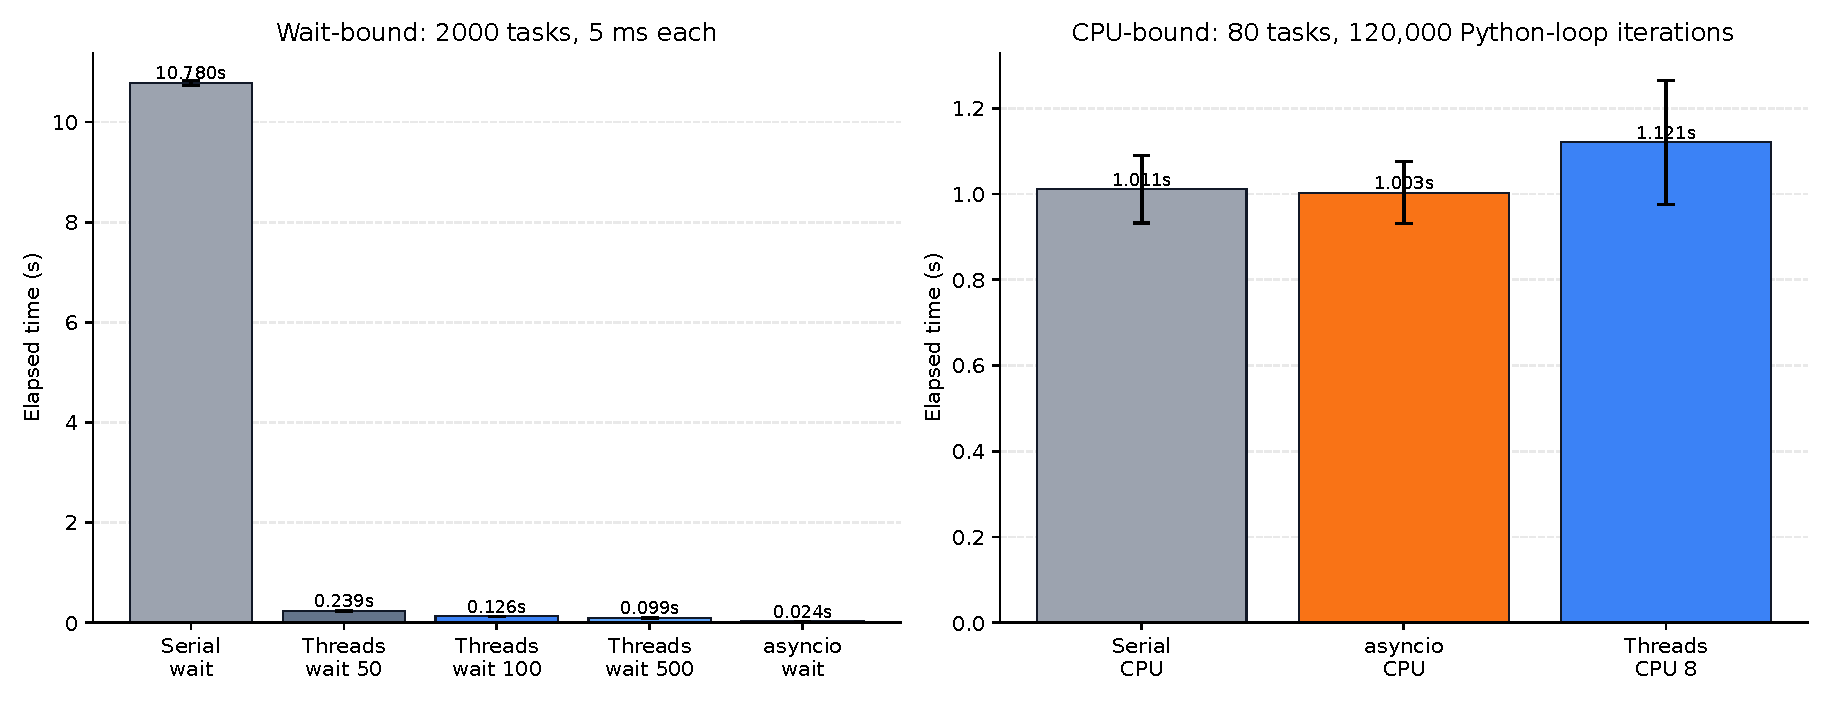
\includegraphics[width=0.94\textwidth]{figures/experiment_benchmarks.pdf}
  \caption{等待型任务与 CPU 密集任务的执行耗时对比}
\end{figure}

\subsection{结果分析}

等待型负载的结果直接支持“等待不应占用线程”这一结论。串行执行接近 $2000 \times 5ms = 10s$；线程池通过并发等待把总耗时降低到 0.1s 到 0.24s 量级，但仍要创建、调度和管理大量 worker。协程版本平均 0.024s，因为 \texttt{asyncio.sleep} 只注册定时等待并挂起当前 Task，事件循环可以继续处理其他就绪 Task，而不是让每个等待任务占住一个 OS 线程。

CPU 密集负载给出的是边界条件。串行版本与 \texttt{asyncio} 版本耗时基本处于同一量级，差异在实验波动范围内；线程池版本没有明显加速，反而略慢。这说明协程任务如果内部没有真实的挂起点，就会在事件循环中顺序占用执行权。对于 Python 纯计算任务，线程池还会受到解释器运行开销和 GIL 等因素影响。该结果与 Java JEP 444 中“虚拟线程不是更快的线程，适合提高吞吐规模而不是让 CPU 计算更快”的判断一致\cite{jep444-notfaster}。

因此，本实验支撑的结论是有限而明确的：协程适合大量等待型任务，因为它把等待状态交给运行时管理；协程不是 CPU 并行计算工具，当任务主要消耗 CPU 时，应考虑多进程、原生扩展、SIMD、GPU 或其他真正能利用多核的并行计算模型。

\section{常见误区与工程注意事项}

\subsection{误区一：协程一定比线程快}

协程的优势主要体现在 I/O 密集型高并发场景。Java JEP 444 明确指出，虚拟线程不是更快的线程，不能让代码运行得比平台线程更快；它们提供的是规模和吞吐，而不是单任务低延迟\cite{jep444-notfaster}。

\subsection{误区二：使用 async 就一定是非阻塞}

\texttt{async} 只是语法标记。真正决定是否非阻塞的是 \texttt{await} 背后的操作。如果在协程中直接调用阻塞 I/O、长时间 CPU 计算或 \texttt{time.sleep()}，事件循环仍然会被卡住。Python 文档也说明，直接在协程中调用阻塞 I/O 会阻塞事件循环，应该使用 \texttt{asyncio.to\_thread()} 等方式把阻塞操作放到其他线程中执行\cite{asyncio-task}。

\subsection{误区三：协程可以替代所有并发控制}

协程降低了并发任务的调度成本，但不会消除共享状态、锁竞争、连接池耗尽、下游限流、取消传播和错误隔离等问题。高质量协程程序仍然需要：

\begin{itemize}
  \item 限制并发度，例如信号量、连接池、限流器；
  \item 正确处理取消和超时；
  \item 避免在事件循环中执行长时间 CPU 任务；
  \item 区分 I/O 密集和 CPU 密集；
  \item 使用 tracing、profiling 和 runtime dump 工具观察调度行为。
\end{itemize}

\section{大语言模型辅助调研过程说明}

本次调研中，大语言模型主要用于资料线索整理和思路校准，不作为直接文献来源。技术事实、实验数据解释和最终文字表述均回到官方文档、手册页和本机实验结果中核对；模型输出只作为待验证线索，帮助更快发现需要阅读或比较的内容。

\subsection{辅助范围}

大语言模型的辅助主要集中在以下几类工作：

\begin{itemize}
  \item \textbf{形成检索关键词}：围绕 coroutine state、async/await state machine、event loop、non-blocking I/O、G-M-P scheduler、virtual thread pinning 等关键词扩展资料检索范围；
  \item \textbf{整理候选资料线索}：先收集可能相关的官方文档或一手资料入口，再逐一打开原文核对，最终只引用确认过的资料；
  \item \textbf{建立对比框架}：梳理语言对比维度，例如编程接口、调度模型、运行时职责、适用场景和工程陷阱，再结合文档内容重写表格和分析；
  \item \textbf{校准实验解释}：围绕“等待型负载”和“CPU 密集负载”区分实验目标，避免把协程的等待调度优势误写成无条件性能优势。
\end{itemize}

本文没有把模型回答直接作为参考文献，也没有直接采用模型生成的结论。涉及 C++20、Python、Go、C\#、Java 21、libuv、Linux epoll/pthreads 等技术事实时，均以官方文档、JEP、语言文档或手册页为准。

\subsection{资料搜集过程}

\begin{center}
\begin{tabular}{p{3.2cm}p{5.4cm}p{5.4cm}}
\toprule
阶段 & 模型辅助内容 & 人工处理方式 \\
\midrule
确定调研范围 & 汇总并发模型演进、协程语义、运行时调度、OS 事件通知、语言对比和实验验证等候选方向 & 保留与协程机制直接相关的部分，形成本文的章节结构。 \\
寻找资料线索 & 汇总 C++20 coroutine、Python asyncio、Go scheduler、Java virtual threads 等主题的资料入口 & 只保留官方文档、OpenJDK JEP、Microsoft Learn、Go 官方源码文档、Linux man-pages 等资料，并逐条核对原文。 \\
提取对比维度 & 梳理编程接口、调度模型、运行时职责、适用场景和工程陷阱等比较维度 & 形成语言对比表；表中具体内容根据原始文档重新整理。 \\
设计验证实验 & 对等待型任务和 CPU 密集任务分别列出可观察指标与可能误读 & 设计两组实验：前者比较 \texttt{asyncio.sleep} 与线程池阻塞等待，后者比较串行、\texttt{asyncio} 和线程池执行纯计算循环。 \\
检查论证边界 & 汇总容易被过度解释的说法，如“协程更快”“async 一定非阻塞”等 & 将“协程不是 CPU 加速工具”“async 不等于非阻塞”“仍需限流和超时”等点纳入工程注意事项。 \\
\bottomrule
\end{tabular}
\end{center}

\subsection{资料核验与最终取舍}

模型输出主要被用作“待核验线索”。例如，资料整理阶段列出了若干需要核验的实现点：Python Task 的协作式调度、C++20 awaiter 接口、Go runtime 的 G-M-P 结构、Java 虚拟线程的 carrier thread 与 pinning 问题。这些内容最终都回到官方文档或一手资料中确认。对于不同资料中的表述差异，本文优先采用更接近运行时实现或标准文档的说法，并避免把“协程更快”这类宽泛表述写成无条件结论。

\section{结论}

协程技术的出现，本质上是为了适应现代服务端高并发、I/O 等待多、请求数量大的工作负载。它通过语言和编译器提供可挂起函数，通过运行时提供任务调度、Future/Task 管理、事件循环和线程映射，通过操作系统提供非阻塞 I/O 和事件通知机制。三者结合之后，程序员可以用接近同步的控制流编写高并发程序。

从语言实现看，C++20 提供最底层、最灵活的 stackless coroutine 机制；Go 通过 Goroutine 和 G-M-P runtime 提供语言级轻量并发；Python asyncio 明确采用单事件循环协作式调度；C\# async/await 与 Task 模型高度整合；Java 21 虚拟线程则选择保留阻塞式代码风格，由 JVM 在底层把虚拟线程映射到平台线程。

最终可以把协程理解为一句话：\textbf{协程不是让计算变快，而是让等待变便宜。} 当系统瓶颈来自大量 I/O 等待时，协程可以显著提高吞吐和资源利用率；当系统瓶颈来自 CPU 计算时，协程并不能替代真正的并行计算模型。

\begin{thebibliography}{99}

\bibitem{cppref}
cppreference.
\newblock Coroutines (C++20).
\newblock \url{https://en.cppreference.com/w/cpp/language/coroutines}

\bibitem{asyncio}
Python Documentation.
\newblock asyncio --- Asynchronous I/O.
\newblock \url{https://docs.python.org/3/library/asyncio.html}

\bibitem{asyncio-eventloop}
Python Documentation.
\newblock Event Loop.
\newblock \url{https://docs.python.org/3/library/asyncio-eventloop.html}

\bibitem{asyncio-task}
Python Documentation.
\newblock Coroutines and Tasks.
\newblock \url{https://docs.python.org/3/library/asyncio-task.html}

\bibitem{concurrent-futures}
Python Documentation.
\newblock concurrent.futures --- Launching parallel tasks.
\newblock \url{https://docs.python.org/3/library/concurrent.futures.html}

\bibitem{pep492}
Python Enhancement Proposals.
\newblock PEP 492 -- Coroutines with async and await syntax.
\newblock \url{https://peps.python.org/pep-0492/}

\bibitem{go-effective}
The Go Programming Language.
\newblock Effective Go: Goroutines.
\newblock \url{https://go.dev/doc/effective_go}

\bibitem{go-faq}
The Go Programming Language.
\newblock Frequently Asked Questions.
\newblock \url{https://go.dev/doc/faq}

\bibitem{go-runtime}
The Go Programming Language.
\newblock Runtime HACKING: Scheduler structures.
\newblock \url{https://go.dev/src/runtime/HACKING}

\bibitem{csharp-async}
Microsoft Learn.
\newblock Asynchronous programming with async and await.
\newblock \url{https://learn.microsoft.com/en-us/dotnet/csharp/asynchronous-programming/}

\bibitem{jep444}
OpenJDK.
\newblock JEP 444: Virtual Threads.
\newblock \url{https://openjdk.org/jeps/444}

\bibitem{jep444-mount}
OpenJDK.
\newblock JEP 444: Scheduling and executing virtual threads.
\newblock \url{https://openjdk.org/jeps/444}

\bibitem{jep444-notfaster}
OpenJDK.
\newblock JEP 444: Virtual threads are not faster threads.
\newblock \url{https://openjdk.org/jeps/444}

\bibitem{oracle-vthreads}
Oracle Java Documentation.
\newblock Virtual Threads.
\newblock \url{https://docs.oracle.com/en/java/javase/21/core/virtual-threads.html}

\bibitem{libuv}
libuv Documentation.
\newblock Design overview.
\newblock \url{https://docs.libuv.org/en/v1.x/design.html}

\bibitem{epoll}
Michael Kerrisk.
\newblock epoll(7) --- Linux manual page.
\newblock \url{https://man7.org/linux/man-pages/man7/epoll.7.html}

\bibitem{pthreads}
Michael Kerrisk.
\newblock pthreads(7) --- Linux manual page.
\newblock \url{https://man7.org/linux/man-pages/man7/pthreads.7.html}

\end{thebibliography}

\end{document}
